% --- [ Recovery of Pre-test Loops ] -------------------------------------------

\subsection{Recovery of Pre-test Loops}
\label{sec:recovery_of_pre_test_loops}

The control flow recovery results of the Hammock method, the Interval method, and for comparison the theoretical optimum when recovering \textit{pre-test loops} (e.g. \texttt{while}-loops) from the combined test programs of Coreutils and SQLite are presented in figure \ref{fig:total_results_pre_loop}.

The \textbf{Hammock method} correctly recovered $29.09\%$ of the pre-test loops present in the test programs (\textit{true positives}). On average, for every $10$ pre-test loops of the original source code, the Hammock method recovered $0.1$ pre-test loops that were \textit{not} present of the original source code (\textit{false positives}).

The \textbf{Interval method} correctly recovered $75.07\%$ of the pre-test loops present in the test programs (\textit{true positives}). On average, for every $10$ pre-test loops of the original source code, the Interval method recovered $4.7$ pre-test loops that were \textit{not} present of the original source code (\textit{false positives}).

Note, at this level of comparison, \textit{pre-test loops} and \textit{infinite loops} are both regarded as pre-test loops. Both the Hammock method and the Interval method distinguish pre-test loops from infinite loops. However, the C parsing script described in step \ref{itm:step_c_to_json} of section \ref{sec:evaluation_process} does not evaluate loop conditions, and can therefore not conclusively determine which conditions are always true (e.g. \texttt{while (TRUE)}). For this reason, no distinction is made between pre-test loops and infinite loops during the evaluation.

\begin{figure}[htbp]
	\centering
	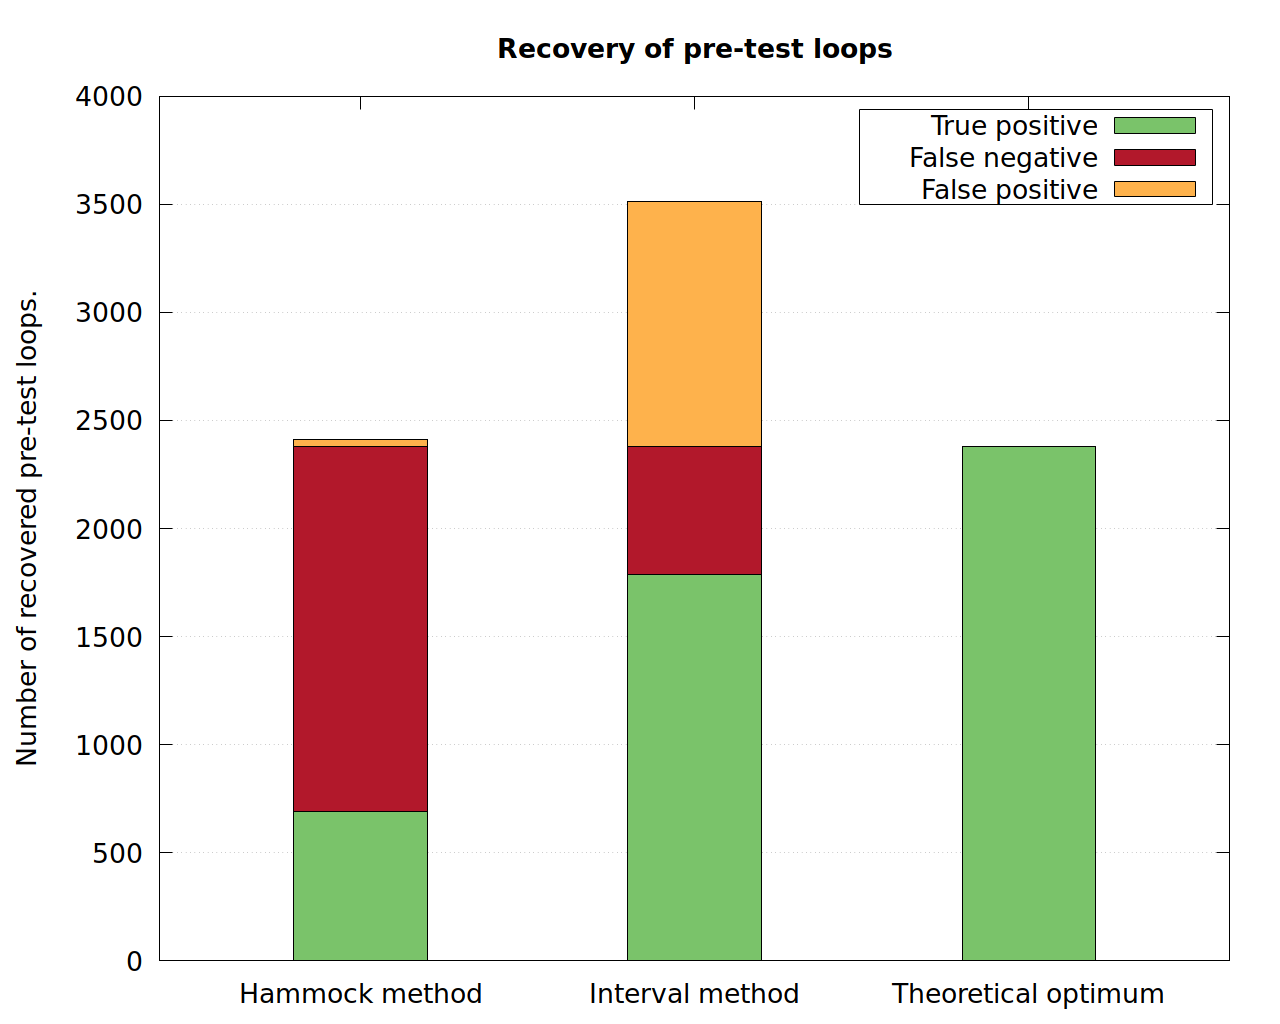
\includegraphics[width=\textwidth]{inc/5_results/results_pre_loop.png}
	\caption{Comparison of control flow recovery results for each method when recovering \textit{pre-test loops}. The data is based on the combined test programs of Coreutils and SQLite.}
	\label{fig:total_results_pre_loop}
\end{figure}
